\documentclass[english]{scrartcl}
\pagenumbering{arabic}
\usepackage[utf8]{inputenc}
\usepackage[english]{babel}
\usepackage{amsmath}
\usepackage{amsfonts}
\usepackage{amssymb}
\usepackage{fancyvrb}
\usepackage{xspace}
\usepackage{refstyle}
\usepackage{hyperref}
\usepackage{listings}
\usepackage{enumitem}
\usepackage{graphicx}

% ============================================================
% Markup macros for proof-reading
\usepackage{ifthen}
\usepackage[normalem]{ulem} % for \sout
\usepackage{xcolor}
\newcommand{\ra}{$\rightarrow$}
\newboolean{showedits}
\setboolean{showedits}{false} % toggle to show or hide edits
%\setboolean{showedits}{false} % toggle to show or hide edits
\ifthenelse{\boolean{showedits}}
{
	\newcommand{\ugh}[1]{\textcolor{red}{\uwave{#1}}} % please rephrase
	\newcommand{\ins}[1]{\textcolor{blue}{\uline{#1}}} % please insert
	\newcommand{\del}[1]{\textcolor{red}{\sout{#1}}} % please delete
	\newcommand{\chg}[2]{\textcolor{red}{\sout{#1}}{\ra}\textcolor{blue}{\uline{#2}}} % please change
}{
	\newcommand{\ugh}[1]{#1} % please rephrase
	\newcommand{\ins}[1]{#1} % please insert
	\newcommand{\del}[1]{} % please delete
	\newcommand{\chg}[2]{#2}
}
% ============================================================
% Put edit comments in a really ugly standout display
%\usepackage{ifthen}
\usepackage{amssymb}
\newboolean{showcomments}
\setboolean{showcomments}{true}
%\setboolean{showcomments}{false}
\newcommand{\id}[1]{$-$Id: scgPaper.tex 32478 2010-04-29 09:11:32Z oscar $-$}
\newcommand{\yellowbox}[1]{\fcolorbox{gray}{yellow}{\bfseries\sffamily\scriptsize#1}}
\newcommand{\triangles}[1]{{\sf\small$\blacktriangleright$\textit{#1}$\blacktriangleleft$}}
\ifthenelse{\boolean{showcomments}}
%{\newcommand{\nb}[2]{{\yellowbox{#1}\triangles{#2}}}
{\newcommand{\nbc}[3]{
 {\colorbox{#3}{\bfseries\sffamily\scriptsize\textcolor{white}{#1}}}
 {\textcolor{#3}{\sf\small$\blacktriangleright$\textit{#2}$\blacktriangleleft$}}}
 \newcommand{\version}{\emph{\scriptsize\id}}}
{\newcommand{\nbc}[3]{}
 \renewcommand{\ugh}[1]{#1} % please rephrase
 \renewcommand{\ins}[1]{#1} % please insert
 \renewcommand{\del}[1]{} % please delete
 \renewcommand{\chg}[2]{#2} % please change
 \newcommand{\version}{}}
\newcommand{\nb}[2]{\nbc{#1}{#2}{orange}}
\newcommand{\here}{\yellowbox{$\Rightarrow$ CONTINUE HERE $\Leftarrow$}}

\newcommand\rev[2]{\nb{TODO (rev #1)}{#2}} % reviewer comments
\newcommand\fix[1]{\nb{FIX}{#1}}
\newcommand\todo[1]{\nb{TO DO}{#1}}
\newcommand\meta[1]{\nbc{META}{#1}{purple}}
\newcommand\jr[1]{\nbc{JR}{#1}{orange}}
\newcommand\nes[1]{\nbc{nes}{#1}{blue}}
\newcommand\on[1]{\nbc{ON}{#1}{red}} % add more author macros here
\newcommand\ewe[1]{\nbc{EWE}{#1}{olive}} % add more author

% ============================================================

\newcommand{\DD}{Dood\-le\-De\-bug\xspace}
\newcommand{\Doodle}{\texttt{Doo.\-dle}\xspace}
\newcommand{\println}{\texttt{Sys\-tem.\-out.\-println}\xspace}

% ============================================================

\begin{document}
\title{DoodleDebug}
\subtitle{A shot-gun marriage between System.out.println and object inspectors}
\maketitle

\begin{abstract}
\meta{Only copied for now.}
Developers need effective ways to inspect and explore the run-time state of programs they are developing and debugging.  Modern debuggers and object inspectors are powerful tools, but they can only be used to explore specific points in the execution where breakpoints have been set. As a result, developers often resort to inserting ``print statements'' in code to log the state at multiple points in the execution. Print statements, however are a `poor man's debugger'', since their output is static and cannot be further explored.
We propose to combine the simplicity of print statements with the graphical sophistication and interaction of modern debugging tools.
\DD is a simple API modeled loosely after Java's \println. Objects that are ``printed'' generate graphical views that can be further explored, and can also be used to navigate back to source code in the IDE.
We introduce \DD and present the results of a usability study that shows that \DD can be very effective for common debugging tasks.
\end{abstract}

\section{Introduction}

For understanding and debugging a program, developers rely on tools to track its runtime states during execution.
One method is to insert print statements like \println in Java.
This method is quick and allows \del{its users} to compare different states in time of a specific object, \ugh{represented by a textual output item}.
However, this output is static and comes with a couple of conceptual restrictions. On the one hand, the level of detail is hardcoded through the textual representations of objects.
If a developer decides for a simple and clear way of representation, they will need to rewrite their code for any further inspection and re-run the program after every change. \nes{That's be a problem in a long-running program.}
If they initially choose a detailed and verbose object representation, the output will grow and become tedious to read.
Another drawback of textual representation is caused by the simplicity of plain text.
It's one-dimensional and contains no information about graphical features like advanced formatting or colors. \nes{Obscure. Colors are a side-dish. What you want to advertise is *nesting*.}

The other half of the two most widely used debugging tools is the family of debuggers~\cite{Kras88a}.
When utilizing a debugger, a program can be stopped at a specific point of its execution, allowing developers to inspect any detail of this very state.
A clear advantage over textual output is the ability to inspect objects on demand.
Information is only displayed as soon as the user asks for it, nevertheless available without re-running the program.
The drawbacks of debuggers arise from the fact that their inspector is always bound to a specific point in time and therefore makes it impossible to directly compare different states of the same object.\nes{Nice.}

\DD combines the power of the above mentioned tools, erasing the conceptual problems coming with them.
Its output is is generated through an API taking its cue from \println's paradigms.
A developer simply needs to call \Doodle(object) to doodle any object type.
For simple customization of object representations, a class can implement the \texttt{Doodleable} interface which contains 2 methods, \texttt{doodleOn} and \texttt{summarizeOn}.
In contrast to Java's \texttt{toString}, there are two methods, allowing developers to create two levels of detail for representation.
This distinction \ugh{takes effect in the principle of Semantic Zoom} \cite{semantic-zoom}.
\ugh{Also, they do not generate plain text but draw content on a virtual canvas.}


\section{Existing Debugging Tools}
\nes{Move to the back, like it was in the paper. I'm a big fan of "related work" in the back of a paper.}
In the world of programming languages, there are two classes of widely used debugging tools:
Textual output like Java's \println and Debuggers.

\subsection{Textual Output}
Java's \println provides a default textual representation for any object, though only primitives and Strings render to a complete (and useful) output in terms of information. \nes{Unnecessarily vague. The rules are no longer than what you're writing: primitives look good; everything else, including arrays!, just gets classname+hashvalue}
\del{Default renderings are kept lean for other objects, but can be easily improved by overriding \texttt{toString}.}
Debugging by directly writing into source code may be easier and quicker than having to equip other debugging tools for a session\ref{some guy}.
Also, objects can be tracked over time, always \ugh{receiving a copy of it} a precisely defined points of execution.

\subsubsection{Best Practice For Textual Output}
For a detailed comprehension of how programmers use textual output for debugging, we wrote a script that searches for such methods in open source projects.
It analyzed SqueakSource, a hosting service for Smalltalk projects, searching for \texttt{printOn} methods, Smalltalk's equivalent to Java's \println.
\todo{Results}

\subsubsection{Missing Features On Textual Output}
Textual output is static.
As a consequence, users always face a trade-off between detail level and compactness.
If the output misses a bit of information, they will need to go back to the code, edit its rendering and re-run the whole program.

Formatting text-only output is restricted to the usage of text characters, tabs and line breaks. \nes{I think we had that nicer in the paper. Why's this a problem? Because it makes it hard to nest layouts. Evidence? We looked at a bunch of system.out.println, and so no nesting going on. This whole paragraph is a re-write of a paragraph in the paper. Maybe steal that one? You're an author after all …}
\ugh{Also, already printed text or line breaks cannot be reverted.
In particular, nesting complex objects in a consistent way is not possible in a trivial way without breaking the whole pattern of \println.}

\begin{figure}[h]
	\begin{lstlisting}
    an Array(
    MatrixTransform2x3(
        2.0 0.0 0.0
        0.0 2.0 0.0
    ) MatrixTransform2x3(
        1 -0.707107 0.0
        0.707107 0.707107 0.0
    ))
	\end{lstlisting}
	\caption{Textual visualization of an array of 2D-matrices, without DoodleDebug.}
	\figlabel{nested-matrix-problem}
\end{figure}

\subsection{Debuggers}
\nes{It's starting to feel very repetitive. DD is positioned between println and Debuggers - fine. Why does that need so many headings and paragraphs?
There's no need to repeat the introduction.}
Debuggers allow users to stop a program's execution at any line of source code.
When stopped, any detail of the current state is inspectable.
Unlike \println, debuggers allow their users to put additional or remove existing break points at runtime, which makes changing the target piece of code to debug quicker, especially because the current program state doesn't need to be re-created like on a new run.

\subsubsection{Drawbacks Of Using A Debugger}
Since a debugger only shows the program's state at one point in time, comparison of two time slices is hardly possible.
Important details may only be memorized and mentally compared to the ones at a later point in time.

Eclipse's built-in Java debugger brings no options to customize its output.
When inspecting an object, all its fields are listed by name, coming along with a textual representation.
An object with many for a programmer unimportant fields may suffer the loss of its clarity from that.


\section{Features}
\todo{more introduction text}
This section summarizes the most important features coming with \DD.
\nes{Sorry for the rant. You can skip it if you want. You're probably best served not reading all of it. But do follow the link by the end!}

\nes{The word "feature" is used correctly here - the things that you describe really are features.
A bit further down, you ask "'Lean API' - does this belong here?". Why, of course. A feature is "a distinctive attribute or aspect of something". Surely, we worked very hard to keep the API simple, so that's our most distinctive attribute. It's also println's most distinctive attribute, so we are competing with println in terms of leanness - this is not only a feature of DD, it is maybe the most important.}

\nes{Given how clear the answer is - why weren't you sure if this belongs here?}

\nes{There's some kind of confusion there, and I see it every time I walk thru an electronics store and the stickers on the items list features -- the longer the list, the higher the price. And the mindset of the sales staff is: "Every customer is different. Some are more demanding than others. You have to ask yourself -- do you need this feature or don't you? If you need it, better take the bigger version that can do more!" Note how "leanness" is never on those stickers. Neither is simplicity.}

\nes{So, these people don't live on the moon, they heard about design, usability and simplicity. But they just think of them as something you can add later, as one more feature. They hear that people want usable stuff. "Very well," they say, "usable it is. Let's build something, and then have a usability expert make it usable."}

\nes{And now you're already going down the wrong direction. We couldn't have made DD as nice as it is without *designing* it to be nice first.}

\nes{Good design and simplicity aren't things you can bolt on late in the game. You either design for them up front, or they'll never be there.}

\nes{So, none of what you say is wrong, but there are a couple of words which betray if a person feels the need for design or not. Designy folks use words like "beautiful" and "simple" -- because that's what their after. Others use the words "usable" and "easy" -- because they think it's the same, and those words are more to the point. But they're not the same. As important as usability is -- it isn't quite the same as beautiful.}

\nes{And simplicity - now, if you suffered thru my boring and longish rant, there's a reeeeally nice talk about the difference that I believe you may enjoy a lot. It's called "simple made easy." www.infoq.com/presentations/Simple-Made-Easy}

\meta{Well, what you describe here is the fact that aesthetics are only a small part of design. This was explicitly mentioned in the books I worked through. So when talking about design, I never meant shiny good-looking things, but usability. Where is this used wrongly?}

\meta{If not "Features", how should this section be called? Properties? DoodleDebug in a Nutshell?}


\subsection{Built-in Renderings}
\DD comes with predefined renderings for a number of commonly used data types in Java.
Those include:
\begin{itemize}[noitemsep]
\item Primitives
\item Arrays
\item Booleans
\item Classes
\item Collections
\item Colors
\item Images (various types)
\item Maps
\item Nulls
\item Objects (default)
\item Strings
\item Tables (rectangular two-dimensional arrays and collections)
\item Trowables
\end{itemize}

\subsection{Usability}
\nes{Maybe there's a latex plugin that can play tv advertisement music while the pdf shows this sentence?}
\meta{You are apple user, right?}
For better debugging experience and efficiency, \DD implements several techniques that should take away non-productive workload from the user.

\subsubsection{Configuration-Free}
A key question in the design of a user interface is the level of configurability exposed to users.
Highly customizable solutions may be better for power users that are very familiar to the software in question.
Other users may always remain on default settings, independent of their fittingness.
We followed the advice of Norman\cite{?} and Buxton\cite{?}, which says not to treat everyone as a designer, but rather take away design decisions from users by creating sophisticated defaults.
As a consequence, there is no settings dialogue or file for \DD.

\subsubsection{Smart Scrolling}
In general, an output console can either move its view port to the bottom when new content is appended or stay where it was before.
\DD implements the scrolling behavior of MUSHClient\footnote{\url{http://www.gammon.com.au/mushclient/}} and mIRC\footnote{\url{http://www.mirc.com}}:
The view port will only be moved to the bottom if it already was before new content was added.
If the user doesn't scroll away from the bottom, they will benefit from notifications about new doodles.
On the other hand, users can scroll up to an old doodle without being bounced away when new objects are doodled.

\subsubsection{Notifications}
\seclabel{smart-focus}
When new objects are doodled, \DD autonomously decides whether to set focus to the \DD output view for user notification or not.
The crucial factor for this decision is the elapsed time since the last doodling.
Focus is gained if more than 4 seconds have passed and always for the first doodle of a program run.

When debugging a program with many output events per second, like a game, there is no sense in always notifying the user.
Either they keep their attention on the output as they see it's rapidly changing, or they work somewhere else in the UI and don't want to be pulled back every time.

Users that debug a program that rarely produces output, like caught exceptions, they probably want to be notified about this event and maybe inspect the new doodle. \nes{Connect with the study.}

\subsubsection{Lean API}
\meta{Does this belong in here?}
The \DD API is lean.
It features three ends for developers to interact with it, though most will only ever use the first two.
\begin{itemize}
\item The \texttt{Doo.dle(Object)} method as a drop-in replacement for \println
\item The \texttt{Doodleable} interface and the associated interface \texttt{DoodleCanvas}, in which objects can define simple custom representations
\item The \texttt{RenderingPlugin} interface, which allows developers to provide powerful custom renderings for any type, based on HTML and CSS; source code access is not required here.
\end{itemize}
Altogether, \DD features no more than 10 public methods.

\subsection{Inspecting Doodled Objects}
One of the main problems of textual output is the universal fact that it's static.
\nes{Again?! This is literally the 4th time that you assert that textual output is static.}
To avoid the trade-off between detail level and compactness, we implemented the principle of \emph{semantic zoom} along with \DD:
Every object features two levels of detail for its rendering.
Objects that are nested into others are not graphically scaled down nor removed, but rendered in its summarized, less detailed  version.

In \DD, objects rendered to nesting levels 0 (doodled ones) and 1 are rendered with full detail; objects of nesting level 2 (inside level 1) show their summarized version.
Clicking on a level 1 object opens a popup window only showing this very object, but with more detail since it's on the new nesting level 0 now.
Level 1 object in this window can again be clicked in order to inspect those.
This can be repeated until any leaf of the object tree is reached.
\Figref{addressbook_whole} shows a doodled address book (on level 0) containing several contacts (on level 1). Clicking on one of them creates a pop-up window, moving the respective contact object to new level 0 (\Figref{addressbook_contact}).

\meta{Is the following paragraph clear enough?}
Navigation between nesting layers inside a pop-up is aided with bread crumbs~\cite{Krug00a} \nes{Page?}, which traces the currently inspected branch of the object graph (\figref{breadcrumbs}).
Any parent doodle in this trace can be clicked to jump to it directly.
When zooming out of the graph this way, the just visited branch is still visible in the breadcrumbs area until the user turns into a new path.

\begin{figure}[h]
	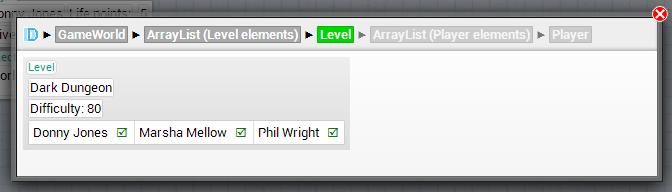
\includegraphics[width=\linewidth]{img/breadcrumbs.png}
	\caption{The labels at the top are \emph{bread crumbs}. The developer is currently looking at a \texttt{Level} object, which is the member of an ArrayList, which is the member of a \texttt{GameWorld}. The object that was doodled was the \texttt{GameWorld} object. The developer was previously zoomed in to player but zoomed out again to Level.}
	\figlabel{breadcrumbs}
\end{figure}

\subsubsection{Tracking an Object Over Time}

Thanks \ins{to} \DD's inspection feature, the summarized representation of an object can be held rather terse.
As an example, the state of a game can be doodled on every update cycle like in \figref{game_long-list}.
A developer observing this output might be interested in more detail of one particular state, which can be done by clicking on parts of it, resulting in a pop-up (\figref{game_last-state}).

The program code defining a \texttt{Player}'s rendering looks as follows:
\begin{lstlisting}
public class Player implements Doodleable {
    public void doodleOn(DoodleCanvas c) {
        c.draw(name);
        c.newLine();
        c.draw("Alive?");
        c.draw(isAlive);
        c.newColumn();
        c.draw("Life points:");
        c.draw(lifePoints);
    }

    public void summarizeOn(DoodleCanvas c) {
        c.draw(name);
        c.draw(isAlive);
    }
}
\end{lstlisting}

\begin{figure}[h]
	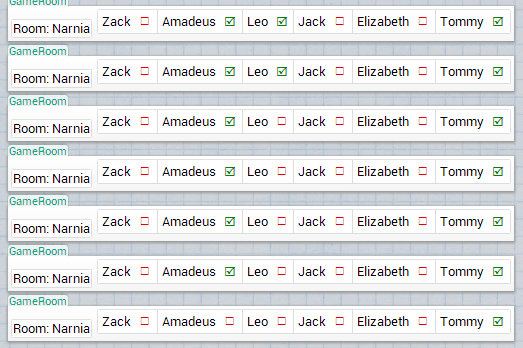
\includegraphics[width=\linewidth]{img/game_long-list.png}
	\caption[Example of a chronological sequence: Game]{A DoodleDebug console showing the doodles of \texttt{GameRoom}s. The boxes beside each are summarized booleans and indicate if the player is alive.}
	\figlabel{game_long-list}
\end{figure}

\begin{figure}[h]
	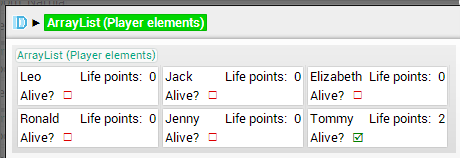
\includegraphics[width=\linewidth]{img/game_last-state.png}
	\caption[Example of a chronological sequence: Detailed player list]{Details of a \texttt{GameRoom} from \Figref{game_long-list}.}
	\figlabel{game_last-state}
\end{figure}

\begin{figure}[h]
	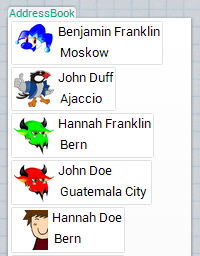
\includegraphics{img/AddressBook_whole.png}
	\caption[AddressBook visualization]{An address book only showing the summaries of its addresses. Clicking reveals the details in \Figref{addressbook_contact}.}
	\figlabel{addressbook_whole}
\end{figure}

\begin{figure}[h]
	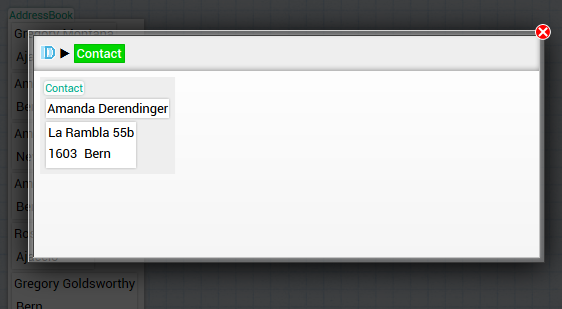
\includegraphics{img/AddressBook_contact.png}
	\caption[Contact visualization]{A popup showing the details of an address.}
	\figlabel{addressbook_contact}
\end{figure}

\subsection{API}
\DD's API features two API layers for customization.
One layer, the Doodleable interface, utilizes a similar paradigm as Java's \texttt{toString()} method and targets most use cases since it's a simple and quick solution.
For more power and flexibility, users may also provide \texttt{RenderingPlugin}s, which are also used internally for \DD's built-in renderings.
However, \texttt{Doodleable} customizations are always preferred over plugins when both are available for a type.

\subsubsection{The Doodleable Interface}

The \texttt{Doodleable} interface features two methods: \texttt{doodleOn(DoodleCanvas)} for a regular representation and \texttt{summarizeOn(DoodleCanvas)} for a simplified and compact version.
Distinguishing between them enables semantic zoom \cite{semantic-zoom} when inspecting doodles.

\paragraph{DoodleCanvas}
Instead of creating a string like in \println, both methods receive a \texttt{DoodleCanvas} object for drawing contents on it.
The paradigm behind \texttt{DoodleCanvas} adopts the formatting of text in terms of lines and columns.
A virtual cursor starts at the upper-left corner of the canvas.
Drawn objects align one beside each other until a new line is created, which causes the cursor to jump back to the left which one line height offset.
The second formatting option is to create new columns, moving the cursor to a position on top, to the right of the right-most previous object.
\texttt{DoodleCanvas} therefore has three public methods: \texttt{draw(Object)}, \texttt{newLine()} and \texttt{newColumn()}.
\Figref{canvas-illustration} shows an example of how the \texttt{Doodleable} interface could be used on a \texttt{Contact} object.

\begin{figure}[h]
	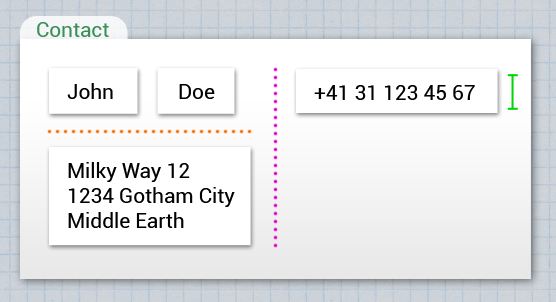
\includegraphics[width=\linewidth]{img/doodleable-example.png}
	\caption[Usage of the \texttt{Doodleable} interface]{Example of a \texttt{Contact} class' \texttt{doodleOn()} method.
Dotted lines visualize the effect of the structuring methods \texttt{newLine()} (orange) and \texttt{newColumn()} (purple).
The green i-beam indicates the final position of the canvas' imaginary cursor.}
	\figlabel{canvas-illustration}
\end{figure}

\subsubsection{Plugins}
There are cases where implementing the \texttt{Doodleable} canvas is not a satisfying option for developers.
If they don't have access to the source code, there is no (clean) way to add an interface.
Also, the \texttt{Doodleable} API only provides rough formatting options.

\paragraph{Implementing Plugins}
For advanced arrangement or additional features like coloring, \DD includes the option to provide plugins.
They must implement \texttt{RenderingPlugin}, which is most easily done by extending the built-in \texttt{AbstractPlugin}.
Each plugin holds information about the object types it is able to render.
Instead of drawing to a virtual canvas, a plugin receives a html \texttt{Tag} object and renders its own HTML code into this tag.
The principle of semantic zoom is again retained through two different methods for different detail levels.
In addition to HTML code generation, plugins have the option to cleanly provide CSS rules and individually adjust class attributes assigned to object doodles.


\section{Design}
\nes{Actually ... Buxton does suggest to mix implementation and design ---- after the initial design is done. He suggests a fading out of design work, as implementation work fades in.}
For the design of \DD's output, we consulted literature to carefully plan the different project cycles.
The most important rule we obeyed was to not mix up design and implementation\cite{?}, which could lead to expensive refactorings or remaining design flaws.	

\subsection{The Sketching Cycle}
\nes{Merge this paragraph with the previous. Outline how this methodology is exactly what Buxton suggests.}
One simple and powerful way to evaluate drafted user interfaces is to confront future users with them.
We took pen and paper and sketched many possible renderings for data types or other UI elements that came to our mind.
As soon as we had accumulated a good amount of them, we internally discussed them to initially get rid of those that obviously contained usability problems.
The other ones were presented to programmers we called over and they had to look at some pictures and explain what they intuitively believed to see (\figref{sketch-discussion}).

\begin{figure}[h]
	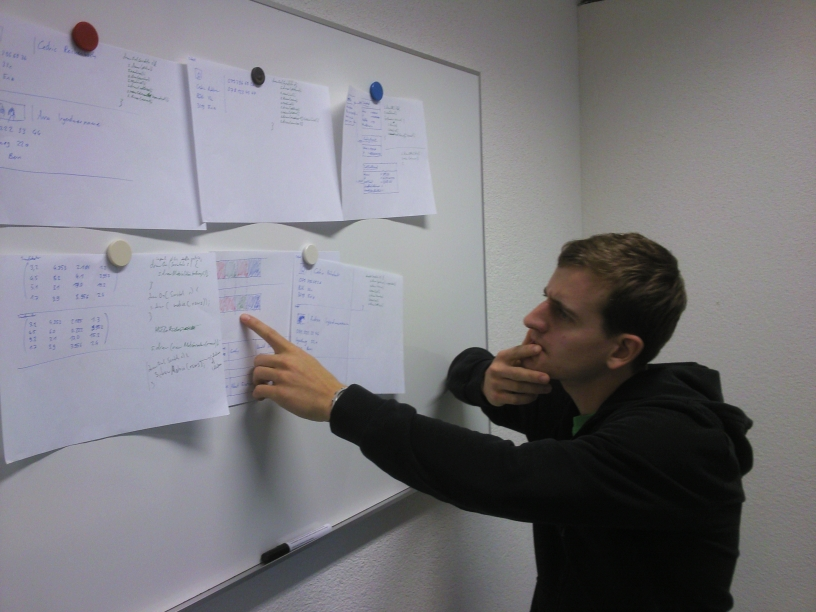
\includegraphics[width=\linewidth]{img/design-sketches_thinker.jpg}
	\caption[Confronting people with design sketches]{Programmer reacting to our sketches.}
	\figlabel{sketch-discussion}
\end{figure}

\begin{figure}[h]
	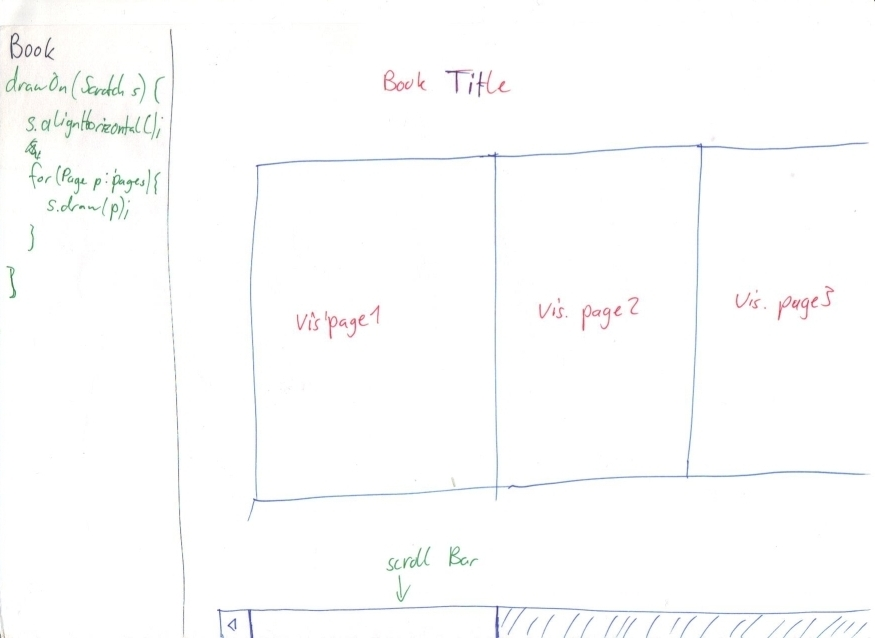
\includegraphics[width=\linewidth]{img/sketches/032.jpg}
	\caption[Bad sketch example: Horizontal and vertical alignment]{Inspired by Swing's FlowLayout, all objects are aligned horizontally.}
	\figlabel{bad-sketch_align-h-v}
\end{figure}

\begin{figure}[h]
	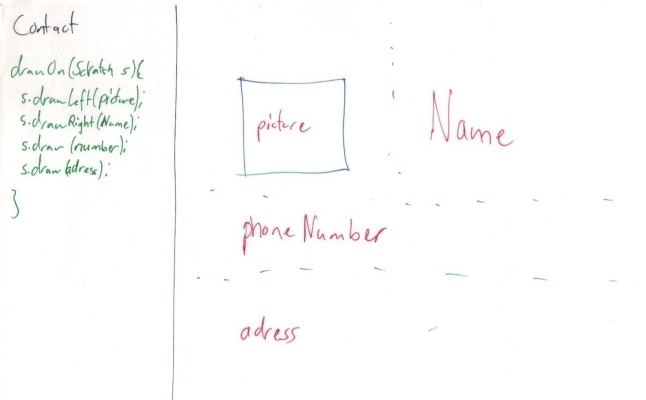
\includegraphics[width=\linewidth]{img/sketches/026.jpg}
	\caption[Bad sketch example: Left-right pattern]{A proposed canvas API that traverses the canvas from top to bottom, dividing it into virtual lines.}
	\figlabel{bad-sketch_left-right}
\end{figure}

If people failed to understand the correct meaning of a sketch, we either improved problematic parts of it or completely refused it.
After improvements or complete re-designs, sketches were presented to other programmers to avoid influencing through the last session.
Sketches that were eventually perceived correctly by most of the people would be accepted for later implementation.


\section{Implementation}
This section outlines the architecture and mechanisms \DD uses in order to perceive data, process them and display the results.

\subsection{Data Transport}
Since \DD is an Eclipse plugin, it's always running in a different Java VM than the project to be debugged itself.
As a consequence, object data needs to be transported after each \Doodle call.
\DD uses a third-party library\cite{xstream} to serialize doodled objects to XML, then transports the result as string over a connection on localhost using SIMON\cite{simon}.

\subsection{Rendering}
After a request for doodling an object has been received, \DD analyzes its type and searches for a fitting rendering in the different customization layers.
If none is available, a default rendering is used.

\subsubsection{Traversing Object Types}
Renderings are iteratively searched for all types and supertypes of an object, starting at the innermost type, defined through the object's class name.
As long as no rendering has been found, the algorithm traverses the inheritance tree in a layer-wise manner, always preferring the class type over interface types inside a layer.
In other words, this algorithm starts searching on the object's direct class and interface types, then goes on for the class' and interface's direct ancestors and repeats until a match was found or all leaves were reached.
The only type excluded from this search is the \texttt{Object} type, since it might be reached before some interface types.

\subsubsection{Output}
As output format, we decided to use HTML.
This enables great formatting possibilities with moderate implementation effort.
Eclipse provides the package \texttt{org.eclipse.swt.browser}, which includes a browser that easily blends into the Eclipse UI.
The rendering used for this browser's content is always the one from the OS's built-in browser and cannot be changed.
On Windows systems, for instace, Eclipse uses the Internet Explorer rendering engine.
As a consequence, we had to be careful when creating HTML output and always test them in different browsers to prevent differences in design on different systems.

\section{User Study}
As we had implemented a new debugging system completely from scratch, we wanted to gather some feedback from potential real world user to verify its usefulness in terms of API and design.
Another goal of such a study would be to reveal problems we might have never found due to our lack of objectivity\cite{the guy that says: "you're not the average user"}.

\subsection{Study Session Setup}
A completely functional release candidate of \DD was used in a fresh Eclipse 4.2 Classic installation, running inside Windows 7 x64 on a ThinkPad T410 with an external mouse.

Since our resources were not unlimited, we decided to do a qualitative study with 7 people as subjects.
We posed 3 different problems to every subject, some of them to be solved with and some without \DD, but with any classical debugging tool they desired.
At the end of the study, we had equally many documentations on problems solved with and without \DD.

Before heading on the study problems, every user had 15-30 minutes to work through a tutorial, play around with \DD in a sandbox and ask questions to the instructor.
When the actual study problems had been revealed, the instructor cancelled their support.

\subsection{Posed Problems}
The 3 different problems aimed on different aspects of debugging in Java.
In the first two problems, the subject was told that a test is failing and they need to find out what the problem is in particular and how to solve it.
For those problems, subjects had full source code access and were allowed to edit anything.

\subsubsection{Sorting}
A couple of gray-scale Color objects are stored in a List.
Some SortingUtil uses a custom comparator with the goal to sort colors by their brightness.
However, sorting the initial color list and comparing it to a hand-built ground-truth list fails.

Solution: The used comparator wrongly treats completely black \texttt{Color} objects as completely white ones.

\subsubsection{Serialization}
A \texttt{SerializingUtil} is used to serialize and de-serialize \texttt{Contact} objects.
Comparison of one particular contact before and after serialization fails.

Solution: The \texttt{long} field \texttt{phoneNumber} in \texttt{Address} as part of \texttt{Contact} changes.
The reason for this is a temporal cast of any \texttt{long} object into an \texttt{int} inside the \texttt{SerializingUtil}.

\subsection{Subjects}
The subjects were convenience-sampled and assured of their anonymity. We informed them about the purpose of our study beforehand, and neither promised nor gave any reward for participating. The participants are enumerated in order of their participation.

\todo{Todo: reduce white space, use a table.}
\meta{Is this still necessary?}
\begin{description}
% Oskar Truffer
\item [{Alpha}] B.Sc in Mathematics, Minor in computer science. Now master student in computer science. % 60 ECTS
% Remo Diethelm
\item [{Bravo}] B.Sc. in Computer Science. Master Student  in Computer Science.
% Andrei Chis
\item [{Charlie}] M.Sc. in Computer Science. Ph.D. Student in Computer Science.
% Julian Schelker
\item [{Delta}] B.Sc. in Computer Science. Master Student  in Computer Science.
% Raffael Krebs
\item [{Echo}] M.Sc. in Computer Science. B.Sc. Working as Software Engineer, 1 year of industry experience. Experience in Eclipse plugin development
% Roger Kohler
\item [{Foxtrot}] B.Sc. in Computer Science. Master Student  in Computer Science.
% Ueli Scheidegger
\item [{Golf}] Lic.rer.pol. in Economics, Minor Computer Science. Working as Software Engineer, 15 years of industry experience. % 60 ECTS
\end{description}

\subsection{Results}
This study revealed information about how programmers come along with \DD, but also how they use classical debugging tools.

\subsubsection{System.out.println}
5 out of 7 subjects used \println for problem solving without \DD.
One argument coming from Alpha was that they were too lazy to change to debug mode.
Furthermore, they stated that comparison between objects was rather helpful for the serialization problem and could not have been done that way with a debugger.

\paragraph{Homogeneous Output}
For finding the problem in the sorting task, Beta printed every color element of the wrongly sorted list to the console.
Afterwards, they stared at the output with numerical color components until they found out the black color is on the wrong end of the list.

In contrast to that, \DD features sophisticated renderings for Collection and Color types, so doodling the list without any customization immediately made the problem obvious.

\paragraph{Uninspectable and Useless Output}
The default implementation of \println prints an object's class name and object hash.
Bravo and Golf cycled between running the program, observing the output and adjusting \println statements to finally reach the part of the object graph they were interested in.

The only subject to override \texttt{toString} methods was Charlie.
They switched from the in this case useless default representation to a solution that lists all fields of an object (\figref{charlie}).

Alpha produced a similar output as Charlie did, but without overriding \texttt{toString}.
Instead, they utilized all getter methods to visualize all fields from outside.

\begin{figure}[h]
\begin{lstlisting}
public class Contact { ...
  public String toString() { 
    return "name: " + name 
        + ", address: " + address;
  }
}
public class Address { ...
  public String toString() {
    return "street: " + street
      + ", phoneNumber: " + phoneNumber
      + ", city: " + city;
  }
}
\end{lstlisting}
  \caption{Custom \texttt{toString()} implementations of a study subject.}
  \figlabel{charlie}
\end{figure}

Another reaction to insufficient output of \println was to immediately switch to a debugger, observed with Bravo and Foxtrott.

\subsubsection{Debugger}
4 out of 7 subjects (Bravo, Delta, Echo, Foxtrott) used the Eclipse debugger for problem solving without \DD, Delta and Echo used it exclusively.
As an advantage over \println, Echo mentioned the inspection features as valuable for comparing two objects like in the serialization problem.
As a second plus, Echo found the simple improvements of textual representations in the debugger useful.
For instance, collections and arrays are rendered as a sequence of their contained elements instead of class name and hash.

\paragraph{Comparison Between Objects}
Directly comparing two objects to approach the source of the serialization problem was done by all subjects except Golf, who immediately started looking at the \texttt{SerializationUtil} source code.

The built-in Eclipse debugger only allows users to inspect one object at a time when using the editor view.
Thus, comparing two objects can become tedious, since one always needs to switch between them and navigate to the relevant part in its graph.
This problem was explicitly pointed out by Echo.

\paragraph{Non-Selective Output}
When inspecting an object, Eclipse's debugger lists all field of an object, since there is no information about their particular relevance.
In particular an object may be referred to through a simple interface in the user-related code.
However, since the debugger is working at runtime, it does not know about the declared type and simply visualizes the instantiated type.
In cases of big classes this can lead to a much more verbose output than the user had expected and therefore complicate inspection.

In our study, we observed this problem in relation to the sorting problem.
Bravo tried to perceive the structure of the color \texttt{List}, which was implemented as an \texttt{ArrayList}.
The resulting representation in the debugger lead Bravo to close the debugger and instead write a for loop, sequentially printing all elements in this list using \println.

\subsubsection{DoodleDebug}
With \DD, none of the problems experienced with other tools were found.
However, we documented a couple of other problems and eventually vanished them during or after the study.

\paragraph{Two Methods in Doodleable Interface}
Echo brought up confusion about the semantic meaning of the two methods in the \texttt{Doodleable} interface.
After going back to the tutorial, he understood.
Without mentioning it, Alpha obviously misunderstood their meaning as well when implementing \texttt{Doodleable} for the first time.
For the smaller representation, they just delegated the zoom by replacing every \texttt{c.draw(object)} method in \texttt{doodleOn} by \texttt{c.drawSmall(object)} in \texttt{summarizeOn}.
Following this observation we removed the \texttt{Canvas.drawSmall} method from the API.

\paragraph{Console Keeps Stealing Focus}
When content is printed to the Eclipse console, it gains focus by default.
The same applied to the \DD output view during the study.
In the initial state of the study problems, they threw an Exception to signal the problem is still unsolved.
When a subject worked with \DD, those two consoles therefore alternatively gathered focus and the view frequently jumped from one to the other.
Every subject experienced this or a similar problem at least once, but only Echo managed to disable this behaviour by clicking a button on the Eclipse console's toolbar menu.

After the study, we implemented a smarter policy to define whether focus should be obtained or not (cf.~\secref{smart-focus}).

\paragraph{Default Doodles Useless}
When investigating an object, study subjects were greatly interested in its instance variables.
Bravo wrote a custom \texttt{toString} method that prints every field of an object labelled with the corresponding field name.
Golf iteratively re-ran the program, each time printing another field of the same object.

After observing this behaviour on the first three subjects, we modified the default object rendering of \DD.
Instead of just utilizing the \texttt{toString} method of an object, the object's fields are listed in its representation unless there are more than 7 declared fields.

\paragraph{Problem Immediately Obvious}
For solving the sorting problem, Charlie doodled both the wrongly sorted list and the manually built ground truth list.
Since they were directly one below each other in the output, he instantly noticed their similarity and their small difference, namely one black element on the wrong end.

Two subjects using \DD on the serialization problem (Delta, Foxtrott) instantly found the problematic field after doodling the contact object before and after serialization.
The reason for this success was that \DD's default object rendering was changed to list all fields of an object, similar to a debugger.


\section{Future Work}
There are a couple of ideas that might enhance debugging experience and efficiency.
However, they'd need to be tested to verify their usefulness, possibly before implementing them.

\subsection{Highlighting Object Diffs}
When tracking and object over time, the most important information is located where properties of an object have changed.
Therefore, a mechanism comparing objects when they are doodled multiple times could be a powerful feature.

\subsection{Clickable Doodles}
One problem of using \println over a long period of time is, that it's indeed clear which object is printed, but not where the \println class has been made.
To find it, some tedious text search over the whole project is needed in the worst case.
As a solution in \DD, doodles could include a link pointing to the line in source code where the \Doodle call was triggered, similar to the way Throwables are tracked.

\subsection{Debugger Integration}
Since the eclipse debugger only uses textual representations and doesn't allow any customization, a way to enhance it could be to include doodles.
A user would be allowed to switch from the standard textual mode to \DD mode, where an object would be inspected using \DD's rendering.
Or a button beside the textual representation would create a popup with the doodled version of it.

\section{Conclusion}
\meta{Was a bit lost in this section, didn't really know what to write.}

\DD is a valuable drop-in replacement for Java's \println.
It introduces techniques to enhance debugging output by adopting well-proven mechanisms from debuggers and console printing on the one hand and introducing simple new ones on the other hand.
Getting started is rather easy since the setup work is mainly done by Eclipse and the API is simple; knowing one single method already enables the core features of \DD.
Continuous migration from classical tools to \DD is not a problem, since parallel usage works flawlessly.

Since the output is held in HTML and \DD is bound to be an Eclipse plugin, the possibilities for additional features are infinite.
The output view with JavaScript running in it is Turing-complete and supports any graphical output a monitor can display.
Any IDE-related actions can be implemented because a stable communication between output and plugin code is already running.

\section{Acknowledgements}

\bibliographystyle{plain}
\bibliography{/bib/scg}
\todo{I can't get it to work... -.-}

\end{document}